\RequirePackage{amsthm} %https://tex.stackexchange.com/questions/687324/unknown-theoremstyle-warning-with-springer-nature-template
\documentclass[sn-mathphys-num,iicol]{sn-jnl}
%\documentclass[sn-mathphys-num,iicol]{jnl}

%\usepackage{sn-jnl.sty}
\usepackage{graphicx}%
\usepackage{multirow}%
\usepackage{amsmath,amssymb,amsfonts}%
\usepackage{amsthm}%
\usepackage{physics}
\usepackage[locale=DE]{siunitx}
\usepackage{mathrsfs}%
\usepackage[title]{appendix}%
\usepackage{xcolor}%
\usepackage{textcomp}%
\usepackage{manyfoot}%
\usepackage{booktabs}%
\usepackage{algorithm}%
\usepackage{algorithmicx}%
\usepackage{algpseudocode}%
\usepackage{listings}%
\usepackage{newtxmath}%
\usepackage{yfonts}
\usepackage{braket}
\usepackage{dsfont}
\usepackage[tiny]{titlesec}%
\usepackage[ngerman]{babel}

\theoremstyle{thmstyleone}
\newtheorem{theorem}{Theorem}
\newtheorem{proposition}[theorem]{Proposition}

\theoremstyle{thmstyletwo}
\newtheorem{remark}{Remark}

\theoremstyle{thmstylethree}
\newtheorem{definition}{Definition}

\raggedbottom

\newcommand{\td}{\text{d}}

\titleformat{\subsection}{}{\thesubsection}{1em}{\itshape}
\titleformat{\subsubsection}{}{\thesubsubsection}{1em}{\itshape}

\begin{document}
        
\title[]{Bestimmung des Quark-Antiquark Potentials in der Hamiltonischen Formulierung der kompakten U(1) Eichtheorie.}
\author*[1]{\fnm{Angelo} \sur{Brade}}\email{s72abrad@uni-bonn.de}
\affil*[1]{Rheinische Friedrich--Wilhelms--Universität, Bonn}

\maketitle
\iffalse
	\abstract{
		\section{Introduction}
		The hamiltonian formulation of lattice gauge theory was first regarded as to costly for reasonable calculations. With the upcomming of quantum computers, we now expect a significant speedup of calculations that can be representet with states. The use of entanglement of these states promisses an exponential improvement. This fact moves the hamiltonian formulation in a point of interest again. For that reason we will revisit this formulation and implement the theory on a classical computer.
		I aim to give a good introduction such that other new students of the field will have a condensed understanding and intuition. The setup will be in the compact U(1) theory, pure gauge, truncated appropiately and reduced from the complete configuration space to a physical configuration subspace through Gauss's Law.
		For the numerical results we will take a look at the expectation value for the plaquette operator and finaly calculate the $q\bar{q}$ potential.
	}
\fi

\iffalse
	\begin{textblock*}{140mm}(32.5mm, 25mm)
		\section{Introduction}
		The hamiltonian formulation of lattice gauge theory was first regarded as to costly for reasonable calculations. With the upcomming of quantum computers, we now expect a significant speedup of calculations that can be representet with states. The use of entanglement of these states promisses an exponential improvement. This fact moves the hamiltonian formulation in a point of interest again. For that reason we will revisit this formulation and implement the theory on a classical computer.
		I aim to give a good introduction such that other new students of the field will have a condensed understanding and intuition. The setup will be in the compact U(1) theory, truncated appropiately and reduced from the complete configuration space to a physical configuration space through Gauss's Law.
		For the numerical results we will take a look at the expectation value for the plaquette operator and finaly calculate the $q\bar{q}$ potential.
	\end{textblock*}
\fi

\begin{strip}
	\section{Introduction}
	The hamiltonian formulation of lattice gauge theory was first regarded as to costly for reasonable calculations. With the upcomming of quantum computers, we now expect a significant speedup of calculations that can be representet with states. The use of entanglement of these states promisses an exponential improvement. This fact moves the hamiltonian formulation in a point of interest again. For that reason we will revisit this formulation and implement the theory on a classical computer.
	I aim to give a good introduction such that other new students of the field will have a condensed understanding and intuition. The setup will be in the compact U(1) theory, truncated appropiately and reduced from the complete configuration space to a physical configuration space through Gauss's Law.
	For the numerical results we will take a look at the expectation value for the plaquette operator and finaly calculate the $q\bar{q}$ potential.

\end{strip}

\,\\[160pt]
\section{Theory}
\subsection{Discretisation}

We start by discretising the positional space into sites and links. The sites are spaced by the lattice spacing $a$. To optain the continuum theory in the limit of $a\rightarrow 0$ we need to introduce the coupling constant $g$\cite{RevModPhys.51.659}.

We associate each site with a corresponding positional vector $\vec{r}=(r_x, r_y)$. On the sites the static charges $Q_{\vec{r}}$ positioned. We associate each link with a corresponding position $\vec{r}$ and a direction $\mu$, where $-\mu$ is its opposite direction. For example with $\vec{r}=(1, 2)$ and $\mu=x$ we would denote the link that points from the site $(1, 2)$ to the $x$ direction. We could denote the same link with $\vec{r}=(2, 2)$ and $\mu=-x$.

On the links are the electric field operators $\hat{E}_{\vec{r},\mu}$ positioned. Each electric field $\hat{E}_{\vec{r}, \mu}$ has the vector potential $\hat{A}_{\vec{r}, \mu}$ as its canonical conjugate variable. Thus
\begin{align}
  [\hat{E}_{\vec{r}_{i}, \mu}, \hat{A}_{\vec{r}_{j}, \nu}]=i\delta^{(3)}(\vec{r}_{i}-\vec{r}_{j})\delta_{\mu\nu}.\label{eq:com}
\end{align}
We construct a unitary operator $\hat{U}_{\vec{r}_{j}, \nu}$ (also called link operator) by using the vector potential as the generator in the Lie algebra $\mathfrak{g}$. Thus through the exponential mapping we get the elements of the Lie group G:
\begin{align}
	\hat{U}_{\vec{r}, \mu} = e^{iag\hat{A}_{\vec{r}, \mu}}.\label{eq:exp}
\end{align}
\\\\
\\[180pt]
The generated Lie group $G=\text{U}(n)$ has the complex matrix elements $\hat{U}_{\vec{r}, \nu}$ of dimension $n\cross n$. By taking $n=1$ we choose the U(1) theory, where the phase, thus our vector potantial, is an element of $\mathbb{R}$. Through equation \ref{eq:com} and \ref{eq:exp} we arrive at
\begin{align}
  [\hat{E}_{\vec{r}_{i}, \mu}, \hat{U}_{\vec{r}_{j}, \nu}]      & =\delta^{(3)}(\vec{r}_{i}-\vec{r}_{j})\delta_{\mu\nu}\hat{U}_{\vec{r}_{j}, \nu},\label{eq:comu1}       \\
  [\hat{E}_{\vec{r}_{i}, \mu}, \hat{U}_{\vec{r}_{j}, \nu}^\dag] & =-\delta^{(3)}(\vec{r}_{i}-\vec{r}_{j})\delta_{\mu\nu}\hat{U}_{\vec{r}_{j}, \nu}\dag. \label{eq:comu2}
\end{align}

To explore the effect of the operators on the states, we choose to be in the electric basis with the basis states $\ket{e_{\vec{r_i}, \mu}}$. The basis is made up of all possible states at the links. We optain
\begin{align}
  \hat{E}_{\vec{r}_{i}, \mu}\ket{e_{\vec{r}_{i}, \mu}}=e_{\vec{r}_{i}, \mu}\ket{e_{\vec{r}_{i}, \mu}}.\label{eq:eig}
\end{align}
Furthermore with equation \ref{eq:comu1}, \ref{eq:comu2} and \ref{eq:eig} we get
\begin{align}
  \hat{U}_{\vec{r}_{i}, \mu}\ket{e_{\vec{r}_{i}, \mu}}      & =\ket{e_{\vec{r}_{i}, \mu}+1}\text{ and}\label{eq:eigu1} \\
  \hat{U}_{\vec{r}_{i}, \mu}^\dag\ket{e_{\vec{r}_{i}, \mu}} & =\ket{e_{\vec{r}_{i}, \mu}-1}.\label{eq:eigu2}
\end{align}
We see the unitary operators, also called linked operators, act as ladder operators.
\subsection{Truncation}
Since each field can be any real value, there are infinitly many possible fields for each link, thus constructing an infinitly dimensional basis. To be computable we truncate the possbile values, such that the basis is finite.

Revisiting the elements of U(1) we see, that they live on the unit circle in the complex plane. By limiting the phase of our exponential mapping in equation \ref{eq:exp} to $[-l, l]$, the phase is now an element of $\mathbb{Z}_{2l+1}$. This also truncates the electric field, such that $e_{\vec{r_i}, \mu}\in[-l, l]$. The unitary operators, which as we saw act as ladder operators to the eigenstates, can now also be expressed as
\begin{align*}
	\hat{U}_{\vec{r}, \mu} \mapsto \begin{bmatrix}
		                               0 & \,\dots\, & \,\dots \, & 0 \\
		                               1 & \dots     & \dots      & 0 \\
		                               0 & \ddots    & \vdots     & 0 \\
		                               0 & \dots     & 1          & 0 \\
	                               \end{bmatrix}, \hat{U}_{\vec{r}, \mu}^{\dag} \mapsto \begin{bmatrix}
		                                                                                    0 & 1          & \dots    & 0 \\
		                                                                                    0 & \vdots     & \ddots   & 0 \\
		                                                                                    0 & \dots      & \dots    & 1 \\
		                                                                                    0 & \,\dots \, & \dots \, & 0 \\
	                                                                                    \end{bmatrix}.
\end{align*}
The unitarity $\hat{U}_{\vec{r}, \mu}\hat{U}_{\vec{r}, \mu}^\dag\neq\mathds{1}$ for this is lot, but can be recovered in the continuum limit of $l\rightarrow\infty$. It is importend to point out, that we annihilate the first (last) state when using $\hat{U}_{\vec{r}}^{\dag}$ ($\hat{U}_{\vec{r}}$).
\subsection{Hamiltonian}
The Hamiltonian for the system was orgininally formulated by Kogut and Susskind \cite{PhysRevD.11.395} and thus since known as the so called Kogut Susskind Hamiltonian. It reads
\begin{align*}
	\hat{H}            = & \hat{H}_E+\hat{H}_B+\hat{H}_m+\hat{H}_{\text{kin}}\text{ with}                                                              \\
	\hat{H}_E          = & \frac{g^2}{2}\sum_{\vec{r}} \left(\hat{E}^2_{\vec{r},x}+\hat{E}^2_{\vec{r},y}\right),                                       \\
	\hat{H}_B          = & -\frac{1}{2a^2g^2}\sum_{\vec{r}} \left(\hat{P}_{\vec{r}}+\hat{P}^\dag_{\vec{r}}\right),                                     \\
	\hat{H}_m          = & m\sum_{\vec{r}}(-1)^{r_x+r_y}\hat{\phi}^{\dag}_{\vec{r}}\hat{\phi}_{\vec{r}}\text{ and}                                     \\
	\hat{H}_\text{kin} = & \frac{i}{2a}\sum_{\vec{r}}\left(\phi^{\dag}_{\vec{r}}\hat{U}_{\vec{r}, x}\phi_{\vec{r}+x}-\text{h.c.}\right)                \\
	                     & -\frac{(-1)^{r_x+r_y}}{2a}\sum_{\vec{r}}\left(\phi^{\dag}_{\vec{r}}\hat{U}_{\vec{r}, y}\phi_{\vec{r}+y}+\text{h.c.}\right).
\end{align*}

Firstly, lets get rid of the part we dont need. At the beginnen we introduced the static charges $Q_{\vec{r}}$. They are called static, since they cant move. We say that they have infinit mass, which implies they wont introduce any field and can not be moved. Thus the fermionic fields $\hat{\phi}_{\vec{r}}$ vanish at all $\vec{r}$. This premiss yields
\begin{align*}
	\hat{H}_{m}=\hat{H}_{\text{kin}}=0.
\end{align*}
The computation can also be done with dynamic charges $\hat{q}_{\vec{r}}$ where the mass and kinetik Hamiltonian will make contributions. In this case a phenomena called doubling problem will rise. A common approach for this problem are staggered fermions. We wont take a look at this and stay in the pure gauge case, where only gauge fields exist.

Now we take a look at the two remaining terms. The so called electric Hamiltonian $\hat{H}_E$ and the magnetic Hamiltonian $\hat{H}_B$. The latter originates from taking the real part of the plaquette operator $\hat{P}_{\vec{r}}$. It is the smallest Wilson loop (a closed loop through the lattice on the link operators) and the oriented product of the link operators, i.e.
\begin{align}
	\hat{P}_{\vec{r}}=\hat{U}_{\vec{r}, x}\hat{U}_{\vec{r}+x,y}\hat{U}^{\dag}_{\vec{r}+y,x}\hat{U}^{\dag}_{\vec{r},y},
\end{align}
where we denote e.g. $\vec{r}+x=(r_x+1,r_y)$. We take the hermitian conjugate of the two latter link operators since all link operators only show in positiv $x$ or $y$ direction and when going through the plaquette we are going against the orientation of the two last link operators. We see that by taking the hermitian conjugate of the plaquette operator, we just go through the plaquette the other way around.

The heuristic explaination of the form of the magnetic Hamiltonian is the following: The Plaquettes, as they are closed loops, are essentially conductor loops that introduce a magnetic moment by Farady's law, that is then measured by the magnetic hamiltonian. % TODO: is this correct?

Last but not least we take a look at the electric Hamiltonian. It is essentially the sum over each lattice site over the square of the electric field. Here we use the electric field operators $\hat{E}^{2}_{\vec{r},\mu}$. But not all of them are free. Gauss's law constraints about the half of them such that the others are truly free. The formulation reads
\begin{align}
  \left[\sum_{\mu=x,y}\left(\hat{E}_{\vec{r},\mu}-\hat{E}_{\vec{r}-\mu,\mu}\right)-\hat{q}_{\vec{r}}-Q_{\vec{r}}\right]\ket{\Psi}=0.
\end{align}
Here we sum over all electric field operators that are linked to a site $\vec{r}$ and are expecting them to be the same as the charge deposited on the site. Only those lattice states $\ket{\Psi}$, which produce this relation, are thus physicaly possible. They live in the physical space $\cal{H}_{\text{ph}}$:
\begin{align}
	\ket{\Psi}\in\cal{H}_{\text{ph}},
\end{align}
where we denote by $\cal{H}$ the space in which a lattice configuration lives. Here the physical Hamiltonian is a subspace of the the complete Hamiltonian.


\section{Implementation}
The code for this work can be accessed via GitHub: \url{https://github.com/valentino-dev/Bachelorthesis/tree/main/src}.
\subsection{Matrix representation}
For the implementation, the lattice is constructed and all operators are placed on their links. Then each entry is calculated:
\begin{align*}
	\bra{i}\hat{H}\ket{j} = & \frac{g^2}{2}\sum_{\vec{r}}\left(e_{\vec{r}, x}^2+e_{\vec{r}, y}^2\right)\delta_{ij}           \\
                          & -\frac{1}{2a^2g^2}\sum_{\vec{r}}\bra{i}\left(\hat{P}_{\vec{r}}+\hat{P}_{\vec{r}}^{\dag}\right)\ket{j}
\end{align*}
with $\ket{i}\in\cal{H}$. Starting with $\bra{i}\hat{P}_{\vec{r}}\ket{j}$:
\begin{align*}
	\bra{i}\hat{P}_{\vec{r}}\ket{j}= & \bra{i}\hat{U}_{\vec{r}, x}\hat{U}_{\vec{r}+x,y}\hat{U}^{\dag}_{\vec{r}+y,x}\hat{U}^{\dag}_{\vec{r},y}\ket{j} \\
	=                                & \bra{i}(\ket{e^{(j)}_{\vec{r}, x}+1}\otimes\ket{e^{(j)}_{\vec{r}+x, y}+1}                                \\
	                                 & \otimes\ket{e^{(j)}_{\vec{r}+y, x}-1}\otimes\ket{e^{(j)}_{\vec{r}, y}-1}                                      \\
	                                 & \bigotimes_\text{rest links}\ket{e^{(j)}_{\vec{r}', \mu'}})                                             \\
	=                                & \Braket{i|k}                                                                                                  \\
	=                                & \delta_{ik}
\end{align*}
The formulation reads as following: State $\ket{j}$ will be transformed by the plaquette operator $\hat{P}_{\vec{r}}$ into some state $\ket{k}$. Thus $\hat{P}_{\vec{r}}$ gets an entry at row $\bra{i}$ and column $\ket{j}$ if, and only if, state $\ket{j}$ is transformed into state $\ket{i}$.

Now knowing $\hat{P}_{\vec{r}}$ in matrix representation, trivially yields $\hat{P}_{\vec{r}}^{\dag}=\left(\hat{P}_{\vec{r}}^{*}\right)^{T}$ and with it the matrix representation of the magnetic Hamiltonian.

On a side note, going through states $\ket{i}$ means, counting up in base $2l+1$ with the link states $\ket{e_{\vec{r}, \mu}}$ being the "digits". This is schematically illustrated in \Cref{tab:steidx}.

\begin{table}[h]
	\begin{tabular}{c|c}
		$i$                       & $\ket{i}=\ket{e_{0}^{(j)}, e_{1}^{(j)}, \dots, e_{N_{\text{l}}-2}^{(j)}, e_{N_{\text{l}}-1}^{(j)}}$ \\
		\hline
		$0$                       & $\ket{-l,-l,\dots, -l,-l}$                                                                          \\
		$1$                       & $\ket{-l,-l,\dots,-l,-l+1}$                                                                         \\
		$\vdots$                  & $\vdots$                                                                                            \\
		$2l$                      & $\ket{-l,-l,\dots,-l,l}$                                                                            \\
		$2l+1$                    & $\ket{-l,-l,\dots,-l+1,-l}$                                                                         \\
		$\vdots$                  & $\vdots$                                                                                            \\
		$(2l+1)^{N_{\text{l}}}-2$ & $\ket{l,l,\dots,l,l-1}$                                                                             \\
		$(2l+1)^{N_{\text{l}}}-1$ & $\ket{l,l,\dots,l,l}$
	\end{tabular}
	\caption{Scheme of state indexing with $N_{\text{l}}\coloneq$ number of links and $e_{m}^{(j)}$ being the value for link $m\in[0, N_{\text{l}}-1]$ ($m$ is bijective to $((x, y), \mu)$) in lattice configuration $j\in[0,(2l+1)^{N_{\text{l}}}]$.}\label{tab:steidx}
\end{table}

With this procedure every combination of states $\bra{i}$ and $\ket{j}$ would have to be checked, which would be very costly. Instead just the transformation $\hat{P}_{\vec{r}}\ket{j}=\ket{k}$ is calculated for every state $\ket{j}$ and set $(\hat{P}_{\vec{r}})_{kj}=1$, i.e. having a contribution at row $\bra{k}$ and column $\ket{j}$.

Gauss's Law not only restricts the electric operators, but also the corresponding link operator on the same link. But here Gauss's Law does not impose a dependency, but rather the dynamical link operators automatically produce physical states, where as the fixed link operators do not act on our physical space anymore, which is why the fixed ones are ignored. With plaquette operators there are normally always four link operators, where as now the plaquette operators are a product of any number of link operators ranging from 0 to 4. Which number it will be is then dependent on the position of the plaquette, i.e. the number of dynamical links it loops through. When a plaquette does not go through any dynamical link operators, it will never produce a physical state and thus can be ignored entirely.

\subsection{Exact diagonalization}
Now having the total Hamiltonian in matrix representation, diagonalization is used to compute the eigenvalues and eigenstates. For this the library \texttt{scipy} \cite{2020SciPy-NMeth} is used. It provides the method \texttt{scipy.sparse.linalg.eigsh}, which is an eigensolver and can be used to calculate the $k$ smallest algebraic (SA) eigenvalues. It uses hermitian sparse row matrices, which speed up the process drastically in comparison to dense non hermitian matrices.

Alternatively, instead of exact diagonalization, one could use tensor networks, or on a quantum computer, a variational quantum eigensolver (VQE).

\subsection{Computational resources}
The disadvantage of the Hamiltonian formulation of the lattice gauge theory, that is its need for computational resources,\cite{Feynman1982} since every link can be in $2l+1$ states and in two dimensions, there are two links for every site. Now depending if periodic boundary conditions (PBC) are being used or not, there are links that connect the sites of opposite sides or not.
The exact number of states for a square $n \cross n$ lattice with PBC would be $N=(2l+1)^{2n^2}$ and without PBC $N=(2l+1)^{2(n^2-n)}$. Only physical states are of interest. Using Gauss's Law imposes constraints and thus restricts the number of total states to only the physical states. So each site introduces a constraint
\begin{align}
  \sum_{\mu=x,y}\left(\hat{E}_{\vec{r}, \mu} - \hat{E}_{\vec{r}, -\mu}\right)\ket{\Psi} = Q_{\vec{r}}\ket{\Psi}.
\end{align}
To check if they are linearly independent, Gauss's Law of all sites is summed up:
\begin{align}
	\sum_{\vec{r}}\sum_{\mu=x,y}\left(\hat{E}_{\vec{r}, \mu} - \hat{E}_{\vec{r}, -\mu}\right)\ket{\Psi} = \sum_{\vec{r}}Q_{\vec{r}}\ket{\Psi}.
\end{align}
Only if the total sum of charges is non zero, linear independency is given. But if the total sum is zero, a redundant constraint arises, which reduces the total number of constraints from $n^2$ to $n^2 -1$. From now on the total charge is always zero, since only lattices with no charges or with a pair of opposite charges are considered.

This limits our total number of electric operators $N_{E}=2n^2$ to only a fraction that is dynamic: $N_{E,\text{dyn}} = n^2+1$. A lattice without PBC has $N_{E}=2(n^2-n)$ and $N_{E,\text{dyn}} = n^2-2n+1$.
The number of physical states for a lattice with PBC is thus
\begin{align}
	N_{\text{ph}}=(2l+1)^{n^2+1}.
\end{align}
And without PBC
\begin{align}
	N_{\text{ph}} & =(2l+1)^{n^2-2n+1}                \\
	              & =(2l+1)^{(n-1)^{2}}\label{eq:pbc}
\end{align}
On a side note, \Cref{eq:pbc} shows, that a $n\cross n$ lattice without PBC has just as many links as a lattice with $(n-1)\cross(n-1)$ lattice with PBC.
Since from the calculations, matrices with size $N_{\text{ph}} \cross N_{\text{ph}}$ are returned, the number of physical states will be a good measure for computation time.
To get an idea on some realistic lattices and their number of physical states, see \Cref{tab:num}.

\begin{table}[h]
	\begin{tabular}{c|c}
		lattice                      & $N_{\text{ph}}$ \\
		\hline
		$2\cross2$, no PBC and $l=1$ & \num{3}         \\
		$2\cross2$, PBC and $l=1$    & \num{243}       \\
		$2\cross2$, PBC and $l=7$    & \num{759e3}     \\
		$3\cross3$, PBC and $l=1$    & \num{59.1e3}    \\
		$3\cross3$, PBC and $l=2$    & \num{9.77e6}    \\
		$3\cross3$, PBC and $l=3$    & \num{283e6}    \\
		$3\cross3$, PBC and $l=4$    & \num{3.49e9}
	\end{tabular}
	\caption{Lattice sizes and their number of physical states.}\label{tab:num}
\end{table}

An advantage is, that most of the elements of the Hamiltonian are zero and only a few are non-zero entries. Thus instead of storing all elements, even those that are zero, only the non-zero entries are being stored by row position, column position and the value. This is called a Compressed Sparse Row (CSR) matrix and will reduce the needed memory drastically.\footnote{Nevertheless a Hamiltonian of a $3\cross3$ lattice with PBC and $l=3$ takes about \SI{150}{GB} to be stored.}

Now that a little intuition for the complexity is obtained, the next step is to continue with the actual computation times. This work will not go into the detail of time complexity, but rather use first hand measurements. The calculations are done on the high performance computing (HPC) cluster Marvin of the University of Bonn. Three computation times are listed in \Cref{tab:times}.\footnote{This assessment was done by using one node with two CPUs of the type Intel Xeon 'Sapphire Rapids' 48-core/96-thread 2.10GHz.}
\begin{table}[h]
	\begin{tabular}{c|c|c}
		truncation $l$ & building $\hat{H}$ & diagonalizing    \\
		\hline
		1              & \SI{1.5}{s}        & \SI{0.27}{s}     \\
		2              & \SI{110}{s}        & \SI{11}{minutes} \\
		3              & \SI{1}{h}          & \SI{5}{h}
	\end{tabular}
	\caption{Computation time for a $3\cross 3$ lattice with PBC.}\label{tab:times}
\end{table}
\Cref{tab:times} confirms the problem, that computation times grow rapidly, and large scale computations are not feasible on classical hardware.

To utilize the HPC to capacity, multiprocessing was introduced. The code was rewritten, such that the calculation of the elements are distributed onto the threads, without distributing to thinly, i.e. launching new threads takes more time then processing, or to dense, i.e. not all cores are utilized.

\section{Results}
\begin{figure}[h]
	\begin{center}
		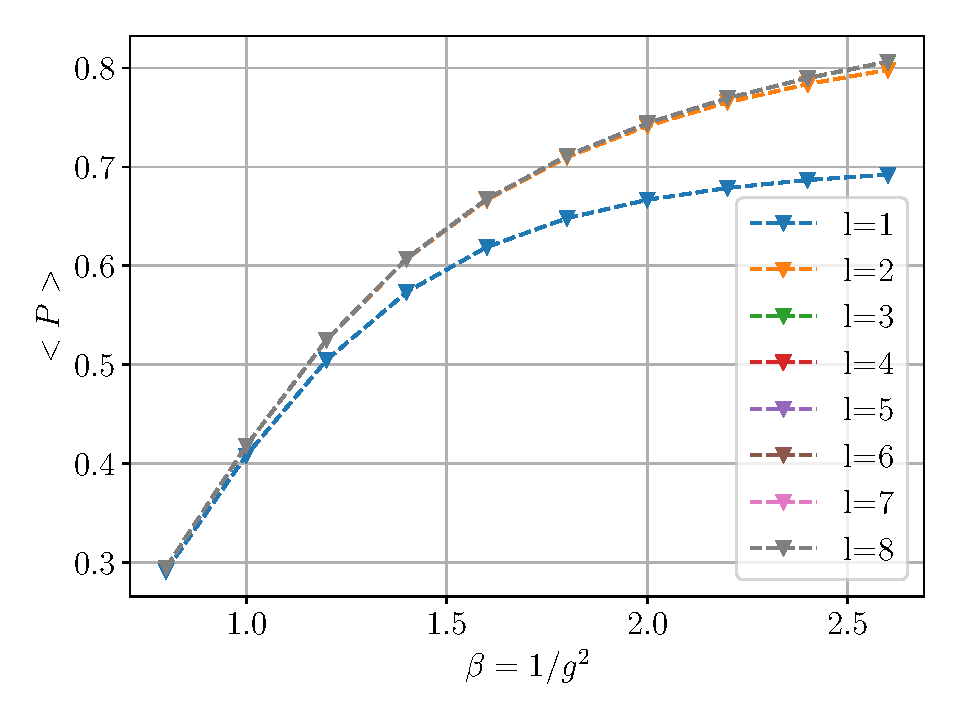
\includegraphics[width=0.45\textwidth]{images/PlaquetteExp2x2.pdf}
	\end{center}
	\caption{plaquette expectation values for a 2x2 lattice.}
\end{figure}
\begin{figure}[h]
	\begin{center}
		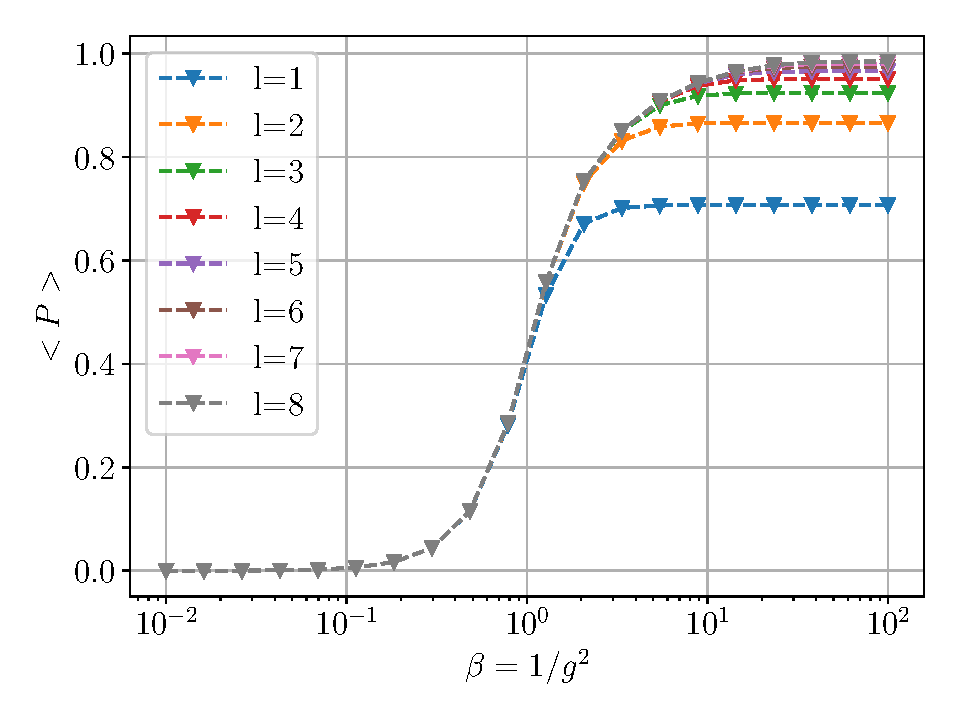
\includegraphics[width=0.45\textwidth]{images/PlaquetteExp2x2Log.pdf}
	\end{center}
	\caption{Plaquette expectation values for a 2x2 lattice in a logarithmic plot.}
\end{figure}
\begin{figure}[h]
	\begin{center}
		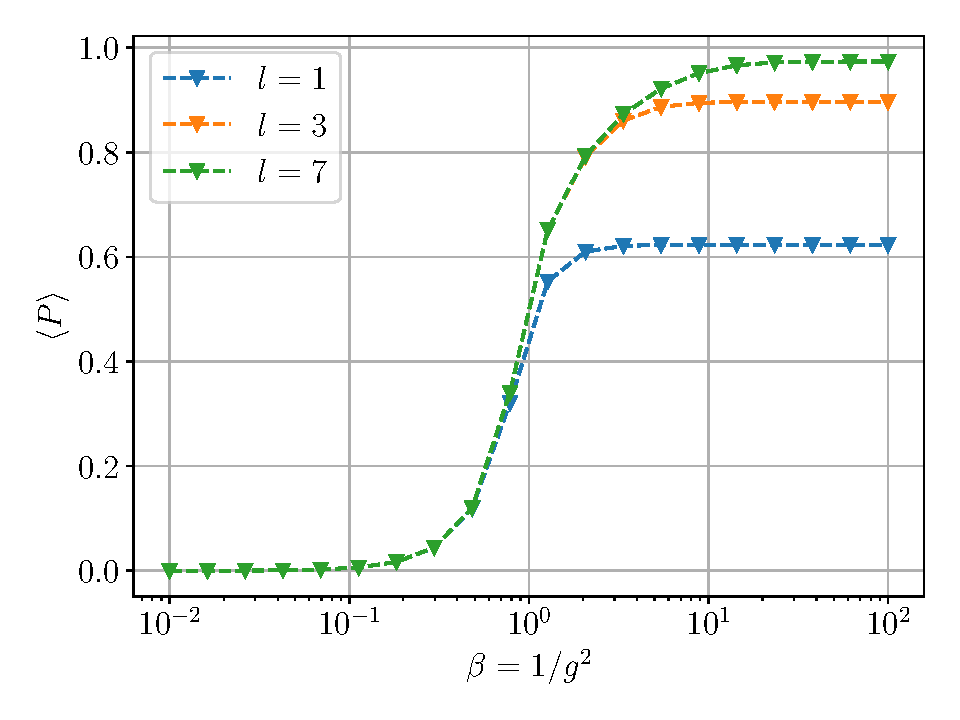
\includegraphics[width=0.45\textwidth]{images/PlaquetteExp2x2PBC.pdf}
	\end{center}
	\caption{plaquette expectation values for a 2x2 pbc lattice.}
\end{figure}
\begin{figure}[h]
	\begin{center}
		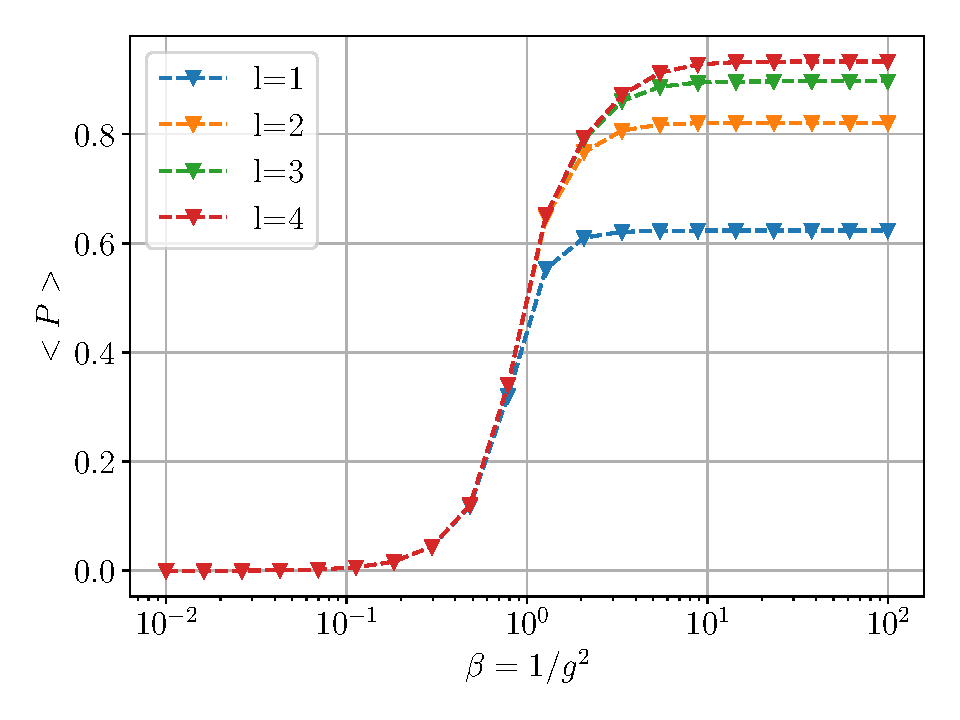
\includegraphics[width=0.45\textwidth]{images/PlaquetteExp2x2PBCLog.pdf}
	\end{center}
	\caption{Plaquette expectation values for a 2x2 pbc lattice in a logarithmic plot.}
\end{figure}
\begin{figure}[h]
	\begin{center}
		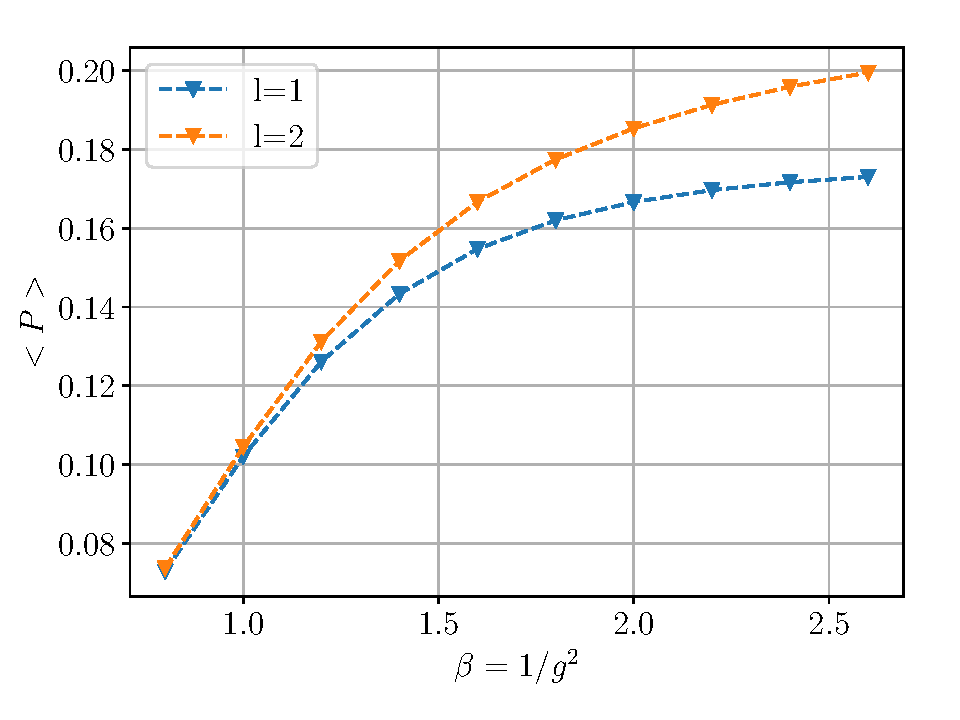
\includegraphics[width=0.45\textwidth]{images/PlaquetteExp3x3.pdf}
	\end{center}
	\caption{Plaquette expectation values for a 3x3 lattice.}
\end{figure}
\begin{figure}[h]
	\begin{center}
		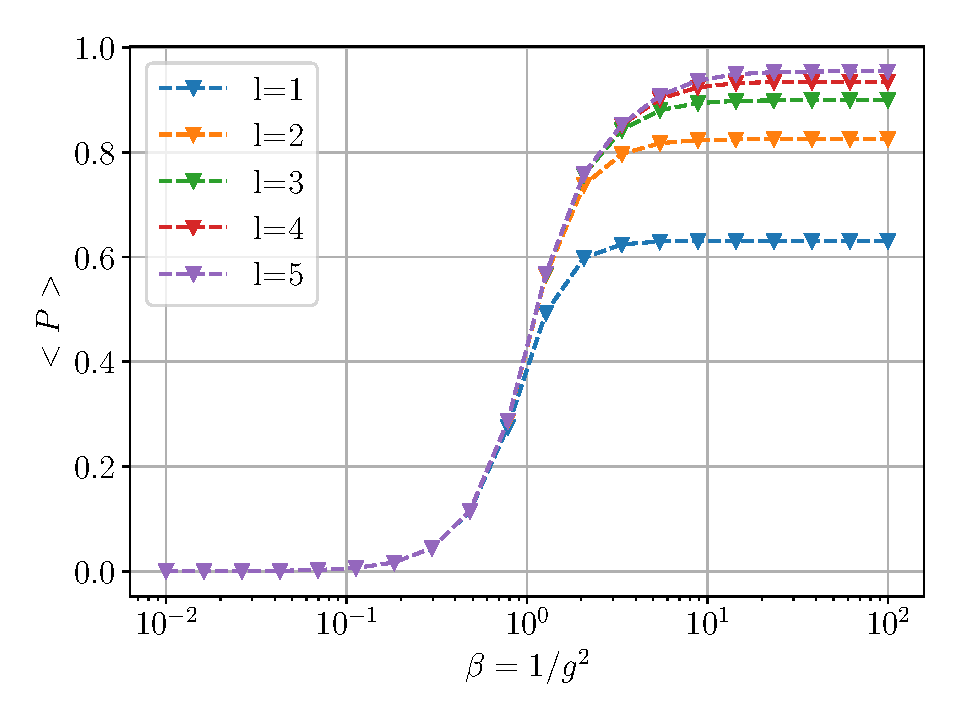
\includegraphics[width=0.45\textwidth]{images/PlaquetteExp3x3Log.pdf}
	\end{center}
	\caption{Plaquette expectation values for a 3x3 lattice in a logarithmic plot.}
\end{figure}
\begin{figure}[h]
	\begin{center}
		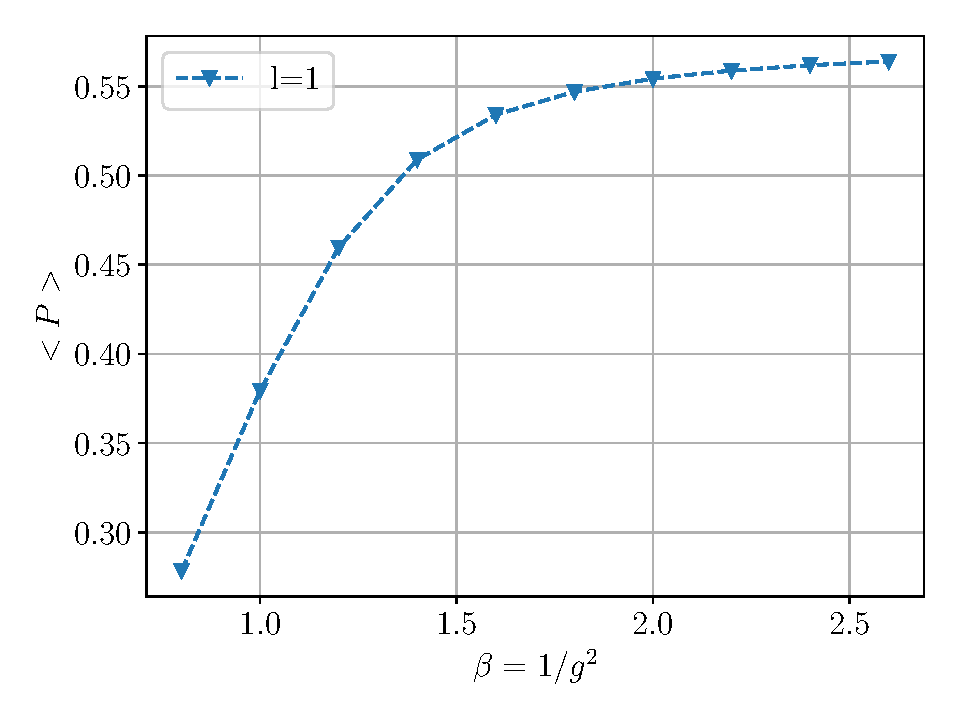
\includegraphics[width=0.45\textwidth]{images/PlaquetteExp3x3PBC.pdf}
	\end{center}
	\caption{Plaquette expectation values for a 3x3 pbc lattice.}
\end{figure}
\begin{figure}[h]
	\begin{center}
		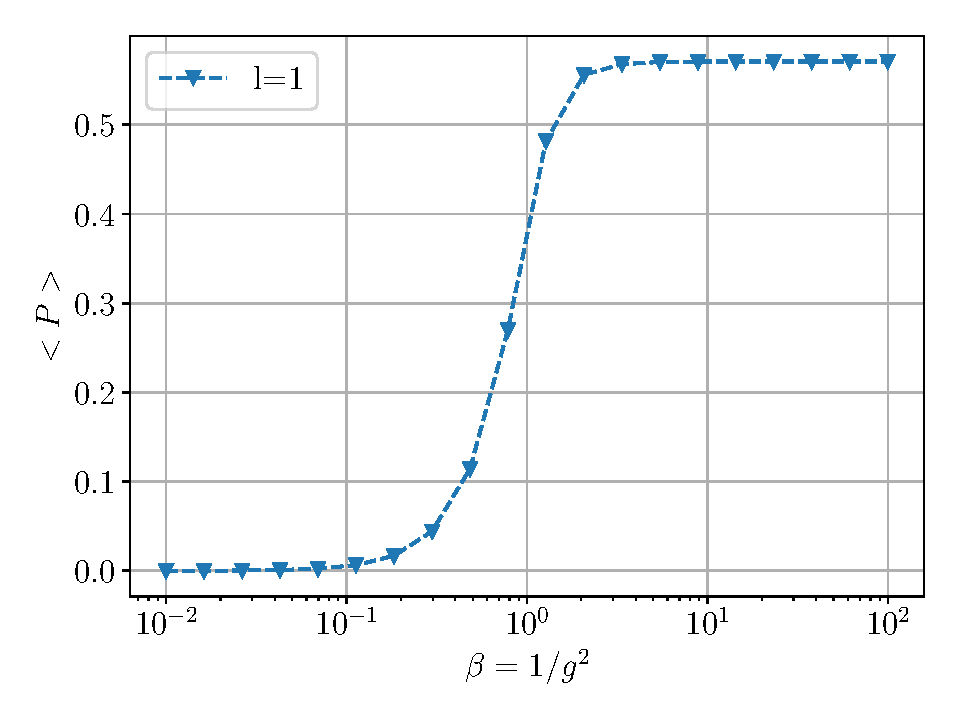
\includegraphics[width=0.45\textwidth]{images/PlaquetteExp3x3PBCLog.pdf}
	\end{center}
	\caption{Plaquette expectation values for a 3x3 pbc lattice in a logarithmic plot.}
\end{figure}
\newpage
fds
\begin{figure}[h]
	\begin{center}
		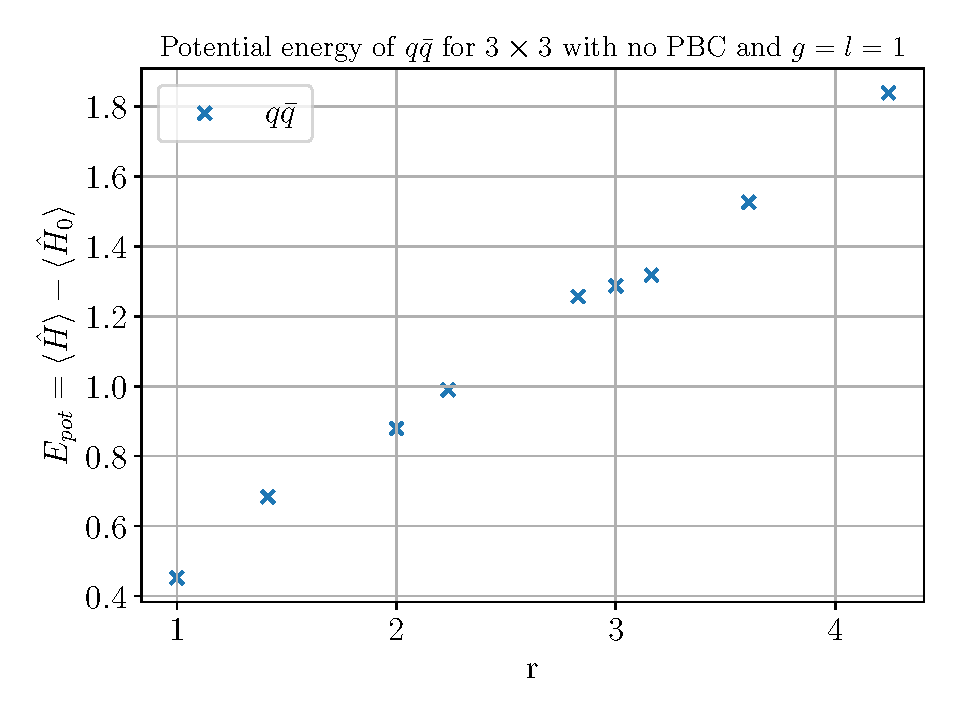
\includegraphics[width=0.45\textwidth]{images/quark-antiquark-potential.pdf}
	\end{center}
	\caption{Quark-Antiquark potential.}
\end{figure}
\begin{figure}[h]
	\begin{center}
		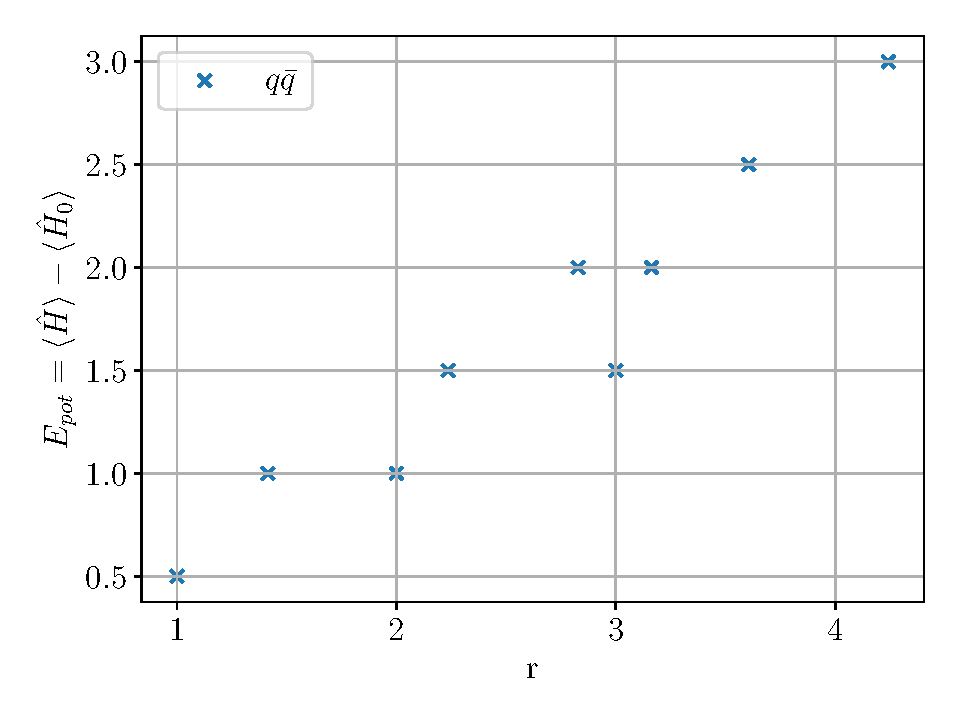
\includegraphics[width=0.45\textwidth]{images/quark-antiquark-potential2.pdf}
	\end{center}
	\caption{Quark-Antiquark potential for 4x4 lattice with l=g=1.}
\end{figure}

\begin{figure}[h]
	\begin{center}
		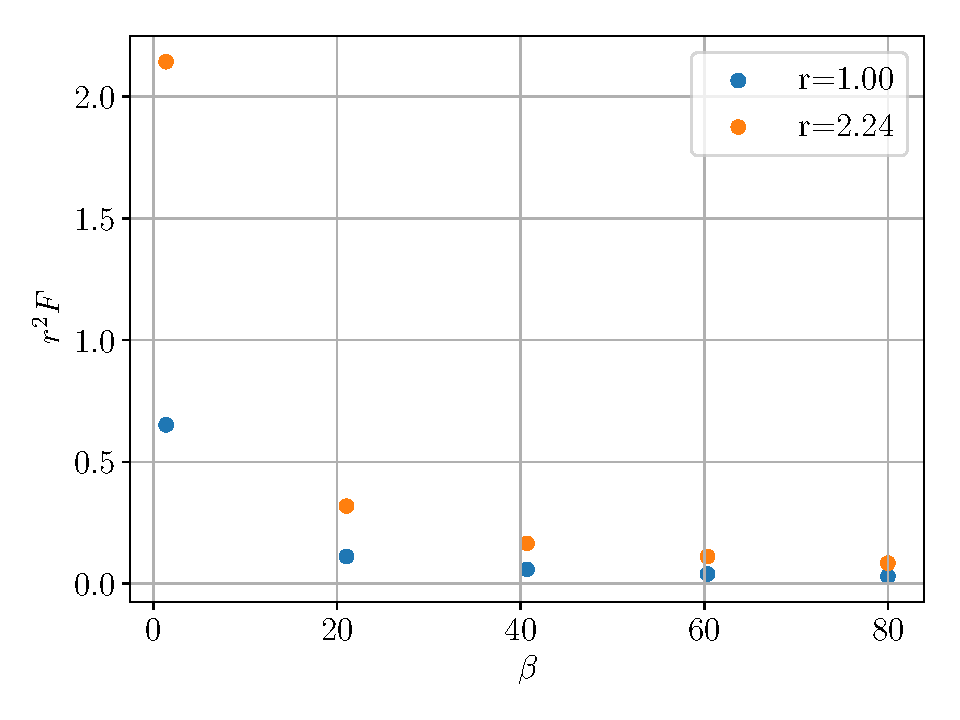
\includegraphics[width=0.45\textwidth]{images/step_scaling.pdf}
	\end{center}
	\caption{Quark-Antiquark potential.}
\end{figure}


\bibliography{refs}
\end{document}
